\RequirePackage{plautopatch}
\RequirePackage[l2tabu, orthodox]{nag}

\documentclass[dvipdfmx]{jlreq}
\usepackage{graphicx}
\usepackage{bxtexlogo}
\usepackage{float}
\usepackage{url}

\title{オブジェクト指向プログラミングレポート課題}

\author{5422007 千本木悠
 5422009 本江拓海 5422020 池田悠星}
\date{\today}

\begin{document}
\maketitle

\section{システムの概要}

\section{クラス設計の指針}

\section{クラス設計の詳細}
\begin{figure}
  \centering
  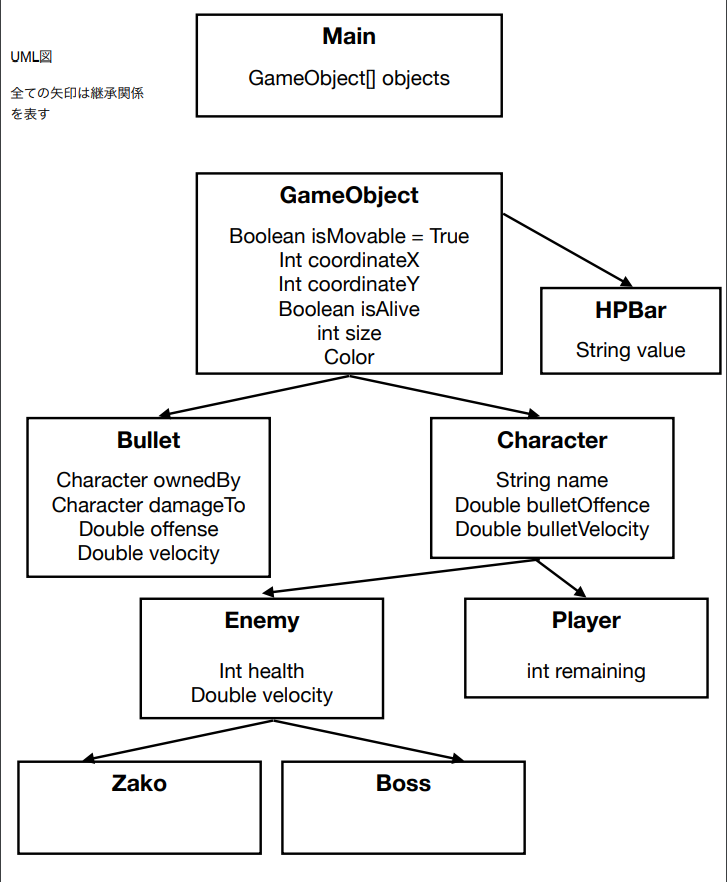
\includegraphics[width=70mm]{figures/class.png}
  \caption{クラス設計図}
  \label{fig:model}
\end{figure}
Mainクラスでゲームのウィンドウや各オブジェクトの設定を行っている.



GameObjectクラスではゲームのオブジェクトを管理する.

HPBarクラスはHPバーを管理する.

Characterクラスでは登場するキャラクターを表す.

BulletクラスではCharacterが打つ弾1つ1つを表す.

Enemyクラスは敵キャラを表す.

Playerクラスはプレイヤーを表す.

--------------
\vskip\baselineskip
Main.java(クラスmain,クラスgamePanel)
\vskip\baselineskip
util.java(クラスutil)
\vskip\baselineskip
GameRegistrer.java(クラスGameRegistrer)
\vskip\baselineskip
GameObject.java(クラスGameObject)
\vskip\baselineskip  
Bullet.java(クラスBullet)
\vskip\baselineskip  
\section{実行結果}

\begin{figure}[H]
\centering
\begin{minipage}[b]{0.32\columnwidth}
    \centering
    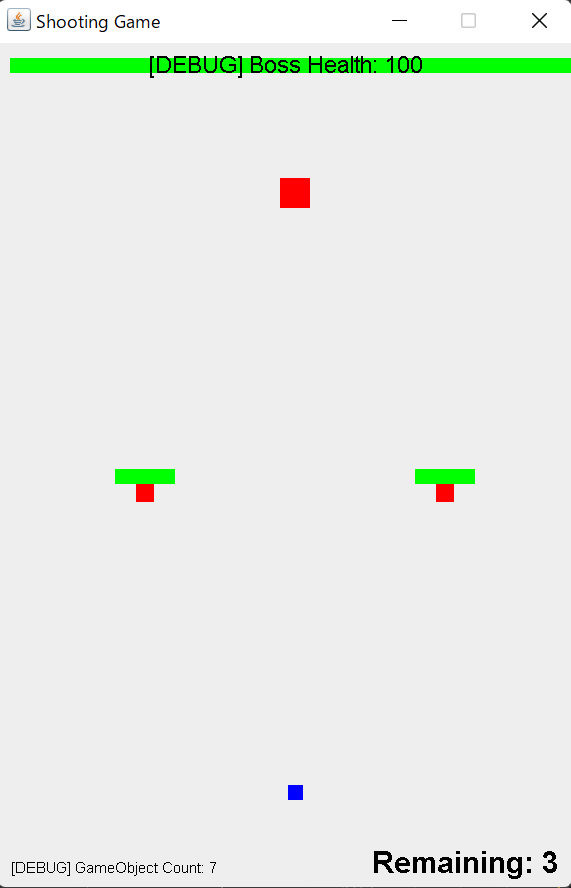
\includegraphics[width=0.7\columnwidth]{figures/result1.png}
    \caption{実行画面1}
    \label{fig:a}
\end{minipage}
\begin{minipage}[b]{0.32\columnwidth}
    \centering
    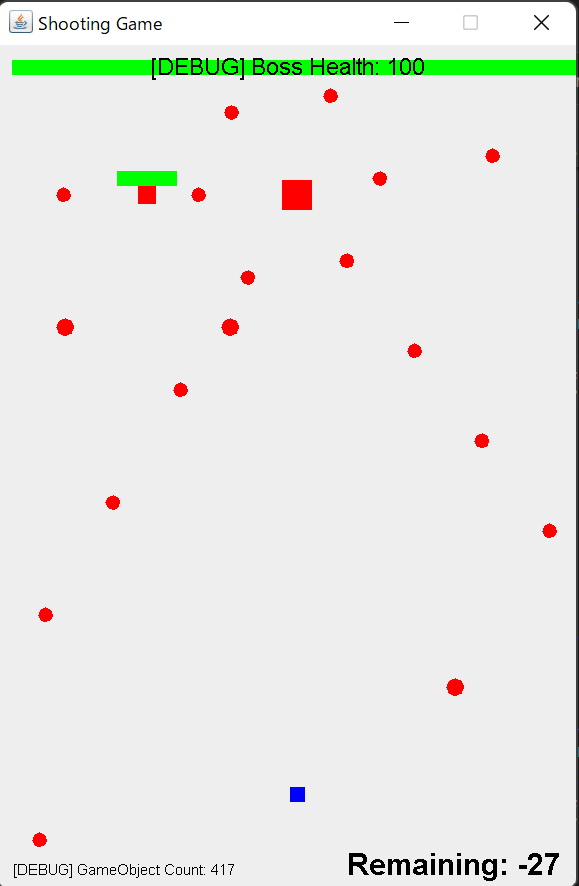
\includegraphics[width=0.7\columnwidth]{figures/result2.png}
    \caption{実行画面2}
    \label{fig:b}
\end{minipage}
\begin{minipage}[b]{0.32\columnwidth}
    \centering
    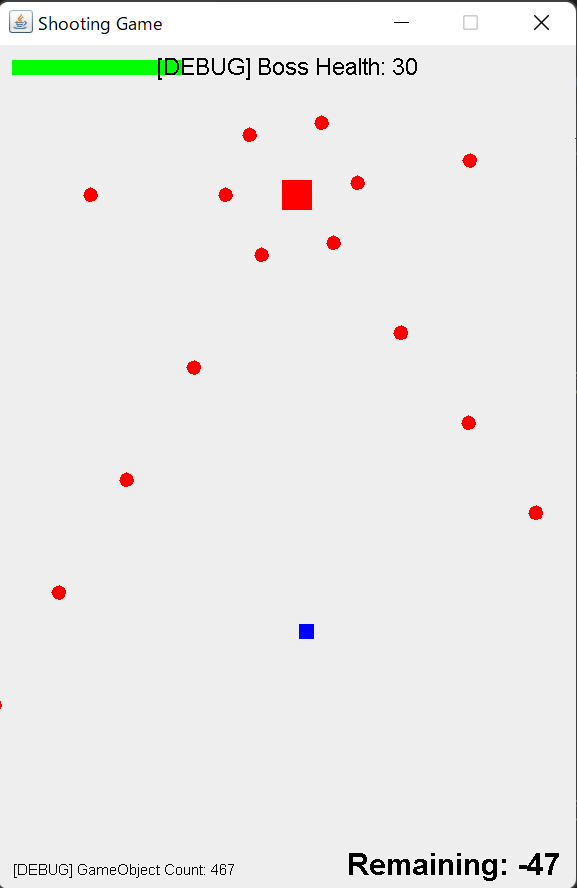
\includegraphics[width=0.7\columnwidth]{figures/result3.png}
    \caption{実行画面3}
    \label{fig:c}
\end{minipage}
\end{figure}

\section{クラス設計に対する考察}

\section{ソースコード}
コードをGitHubに掲載した.URLを以下に示す.

\url{https://github.com/Piertotum-Locomotor/kthr_shooting}
\section{担当箇所}

\end{document}
